%!TEX root = ../thesis.tex
%*******************************************************************************
%****************************** Second Chapter *********************************
%*******************************************************************************

\chapter{Results}
\label{chapter:experiments}

\graphicspath{{../img/plots/vae_latents/}{../img/plots/kodak_comparison/}{../img/plots/kodak_coding_time/}{../img/plots/kodak_side_info/}}

\label{sec:experimental_results}
\par
In this section we detail how we setup and empiricall show the correctness and
the efficiency of our model. We compare our results against JPEG, the most
widely used lossy compression method \cite{bull2014communicating}, and the
current state-of-the-art, the results of \cite{balle2018variational}\footnotemark.
\cite{zhao2015loss}

\footnotetext{We thank the authors of the paper for making their data available
  to us.}

\paragraph{Note:} All experiments were run on a GeForce GTX 1080 GPU.

\section{Experimental Setup}
\par
As we based our models on that of \cite{balle2016end} and
\cite{balle2018variational}, we mirror a lot of their training setup as well
(See Section \ref{sec:dataset_preproc} for the dataset and preprocessing). We
trained all our models with Adam with a starting learning rate of $\alpha_0 =
3 \times 10^{-5}$ and trained all of our models for 20 epochs or equivalently,
approximately 200,000 iterations.. We used a smooth
exponential learning rate decay schedule except in the case of the
$\gamma$-VAEs, according to the formula
\[
  \alpha(t) = \alpha_0 \times r^{\frac{t}{D}}.
\]
Where $r$ is the decay rate, $D$ is the decay step size and $t$ is the current
batch number. We found $r = 0.96$ and $D = 1500$ worked well for our
experiments. We note, however, that we did not notice signifcant performance
gains by using this schedule compared to just using a fixed one.
\par
A surprising result is that even though we have not trained our models for
nearly as long, or on nearly as much data as \cite{balle2018variational}, our
method still gets reasonably close to their results. We compare our results to
theirs, which as far as we are aware are the current state-of-the-art on both
the MS-SSIM and PSNR perceptual metrics.

\section{Comparison of our method with other algorithms}
\par

We present the rate-distorsion curves for the following:
\begin{itemize}
\item JPEG, with quality settings from 1 to 92, with increments of 7 between
  settings. As this is the most widely used lossy image compression codec, it is
  crucial to demonstrate that our method is at least competitive with it, and
  ideally beats it.
\item BPG\footnotemark with 4:4:4 chroma sampling, as we are comparing against
  RGB-based compression techniques. We used quantization settings between 51 to
  33 wiht decrements of 3 between settings.
\item Two models with the same architecture from \cite{balle2018variational},
  one optimized for a MSE training objective, and one optimized for the
  MS-SSIM perceptual metric.
\item Two of our models, all of which were optimized with Laplacian likelihoods,
  one PLN and one $\gamma$-PLN. We plot both their theoretically optimal
  performance as well as their actual performance, with the differences
  explained below.
\end{itemize}

\par
For our method, for each model we present two results: the \textit{theoretically
optimal} performance, and the \textit{actual} performance. The theoretically
optimal BPP was calculated using the theoretically achievable upper bound for
the compression size in bits as given by \cite{harsha2007communication},
without the constant term:
\[
  \I[\vec{x} : \vec{z}] + 2 \log \left( \I[\vec{x} : \vec{z}] + 1\right).
\]
The optimal reconstruction error was calculated by passing an image through the
VAE regularly, instead of using the coded approximate sample. Thus, any
actual method's performance using the same setup must apper to the right of (less
efficient compression) or below (worse reconstruction quality) the theoretical
position.

\footnotetext{We used the implementation available at \url{http://bellard.org/bpg}}

We trained the PLNs using $\beta = \{0.01, 0.03, 0.1, 0.3, 1\}$ and the
$\gamma$-PLNs using $\beta = \{10, 3, 1, 0.3, 0.1\}$.

Our results can be seen in Figure \ref{fig:kodim01_comp}. We observe a similar
phenomenon as \cite{balle2018variational}: there is a mismatch in the comparison
of models according to different perceptual metrics, depending on what objective
they have been optimized for. In particular, JPEG and BPG have both been
optimized so that they give high PSNR (thus, low MSE), whereas they underperform
on the newer MS-SSIM metric. We note that as MS-SSIM correlates better with what
the HVS perceives, we find it more important to do well on that comparison.
\par
In interesting note, that also justifies our choice of the MAE as the training
objective, is the fact that our model optimized for it does well on this metric.

\begin{figure}
  \centering
  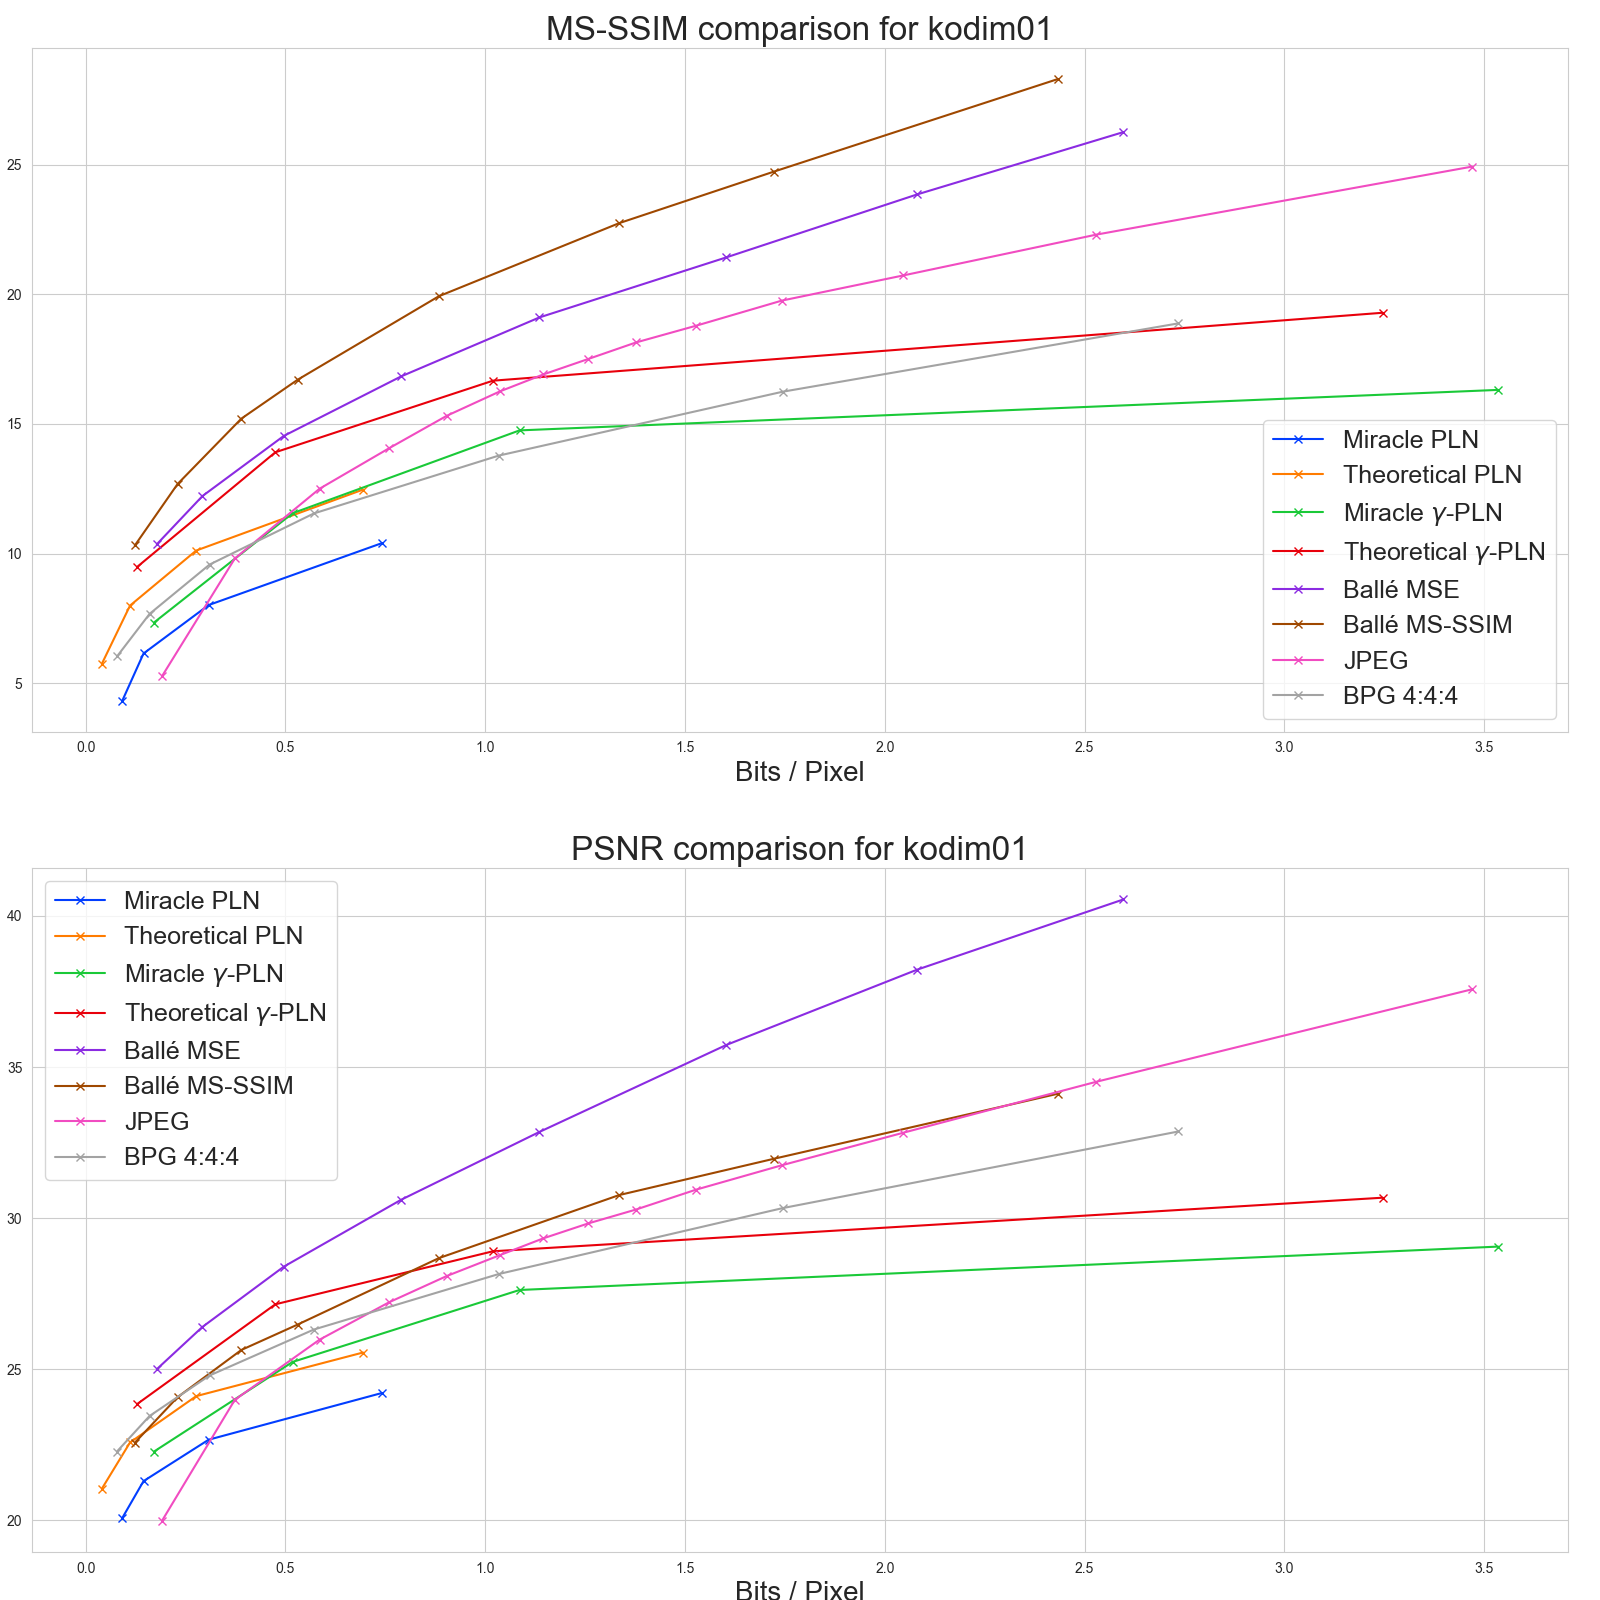
\includegraphics[width=\textwidth]{kodim01_comparison.png}
  \caption{Rate-Distorsion curves of several relevant methods. Please see
    Section \ref{sec:experimental_results} for the description of how we
    obtained each curve. We note that the MS-SSIM results are presented in
    decibels, where the conversion is done using the formula $-10 \cdot
    \log_{10}\left( 1 - \text{MS-SSIM}(\vec{x}, \hat{\vec{x}}) \right)$.
    The PSNR is computed from the mean squared error, using the formula 
    $-10 \cdot \log_{10}\text{MSE}(\vec{x}, \hat{\vec{x}})$.}
  \label{fig:kodim01_comp}
\end{figure}

\section{Analysis of the contribution of the second level}
\par
An important part of verifying the validity of using PLNs is to analyze the
contribution of the second level. Here we look at
\begin{itemize}
\item its contribution to the codelength
\item its efficiency in capturing dependencies between the first level latents
\end{itemize}

\begin{figure}
  \centering
  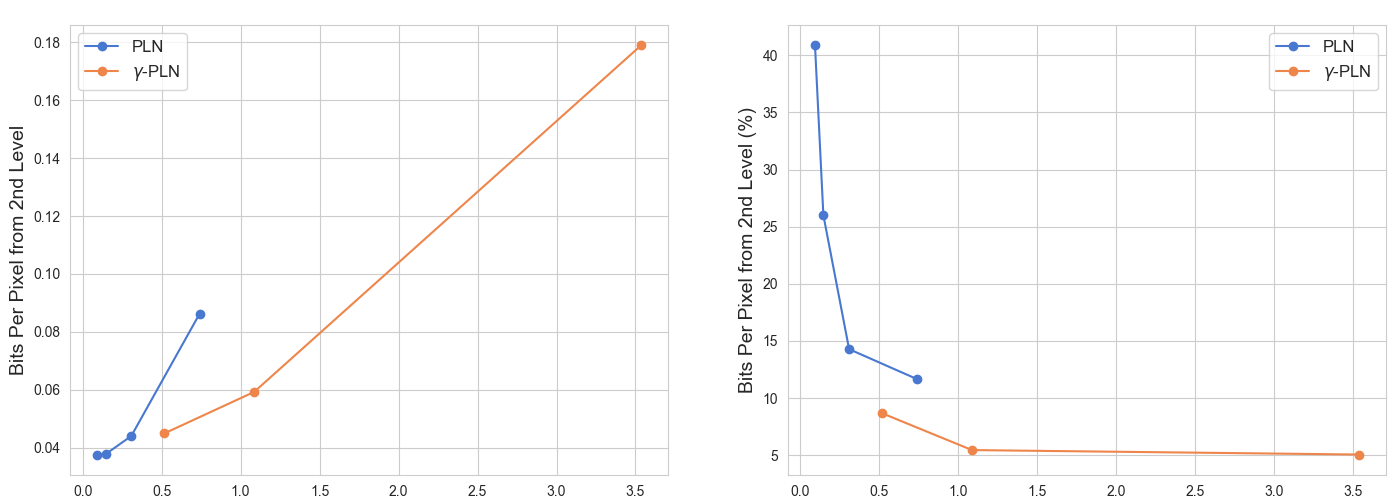
\includegraphics[width=\textwidth]{kodim01_side_info.png}
  \caption{Contribution of the second level to the rate, plotted agains the
    actual rate. \textbf{Left:} Contribution in BPP, \textbf{Right:}
    Contribution in percentages. We see that for lower bitrates there is more
    contribution from the second level and it quickly decreases for higher
    rates. It is also clear that on the same bitrates, the $\gamma$-PLN requires
    less contribution from the second level than regular PLN.}
  \label{fig:kodim01_side_info}
\end{figure}

\begin{figure}[H]
  \centering
  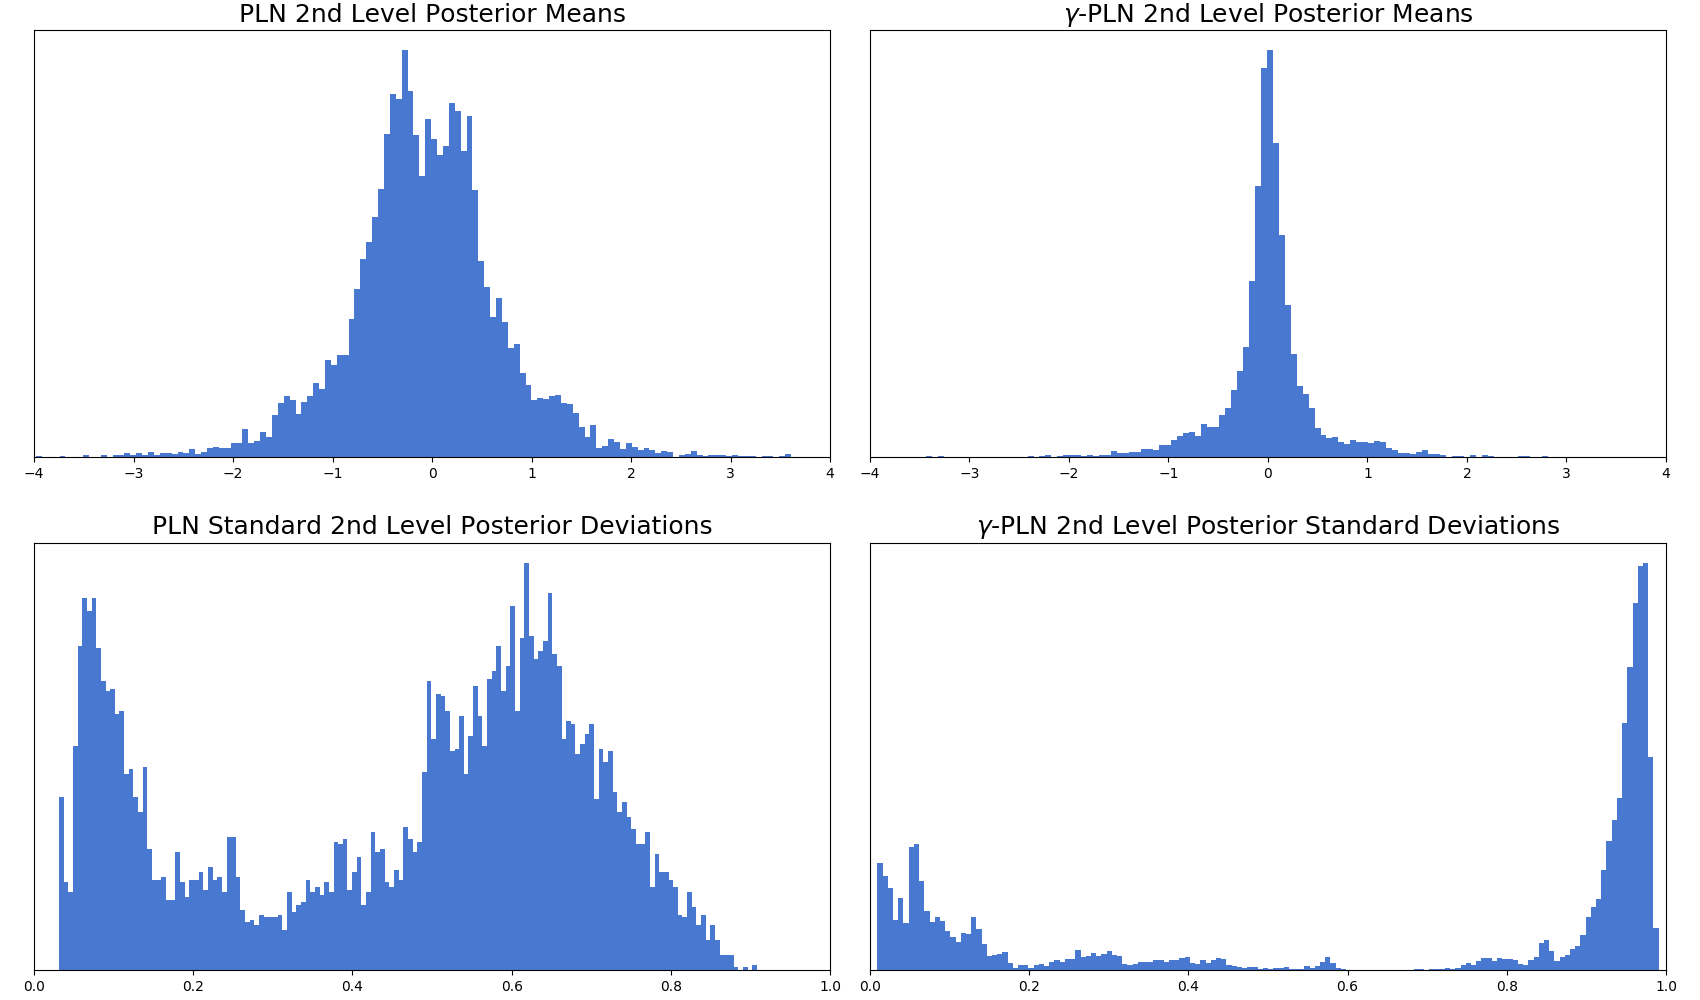
\includegraphics[width=\textwidth]{ladder_gamma_q2_comp.png}
  \caption{ladder on kodim21}
  \label{fig:ladder_gamma_q2_comp}
\end{figure}
\begin{figure}[H]
  \centering
  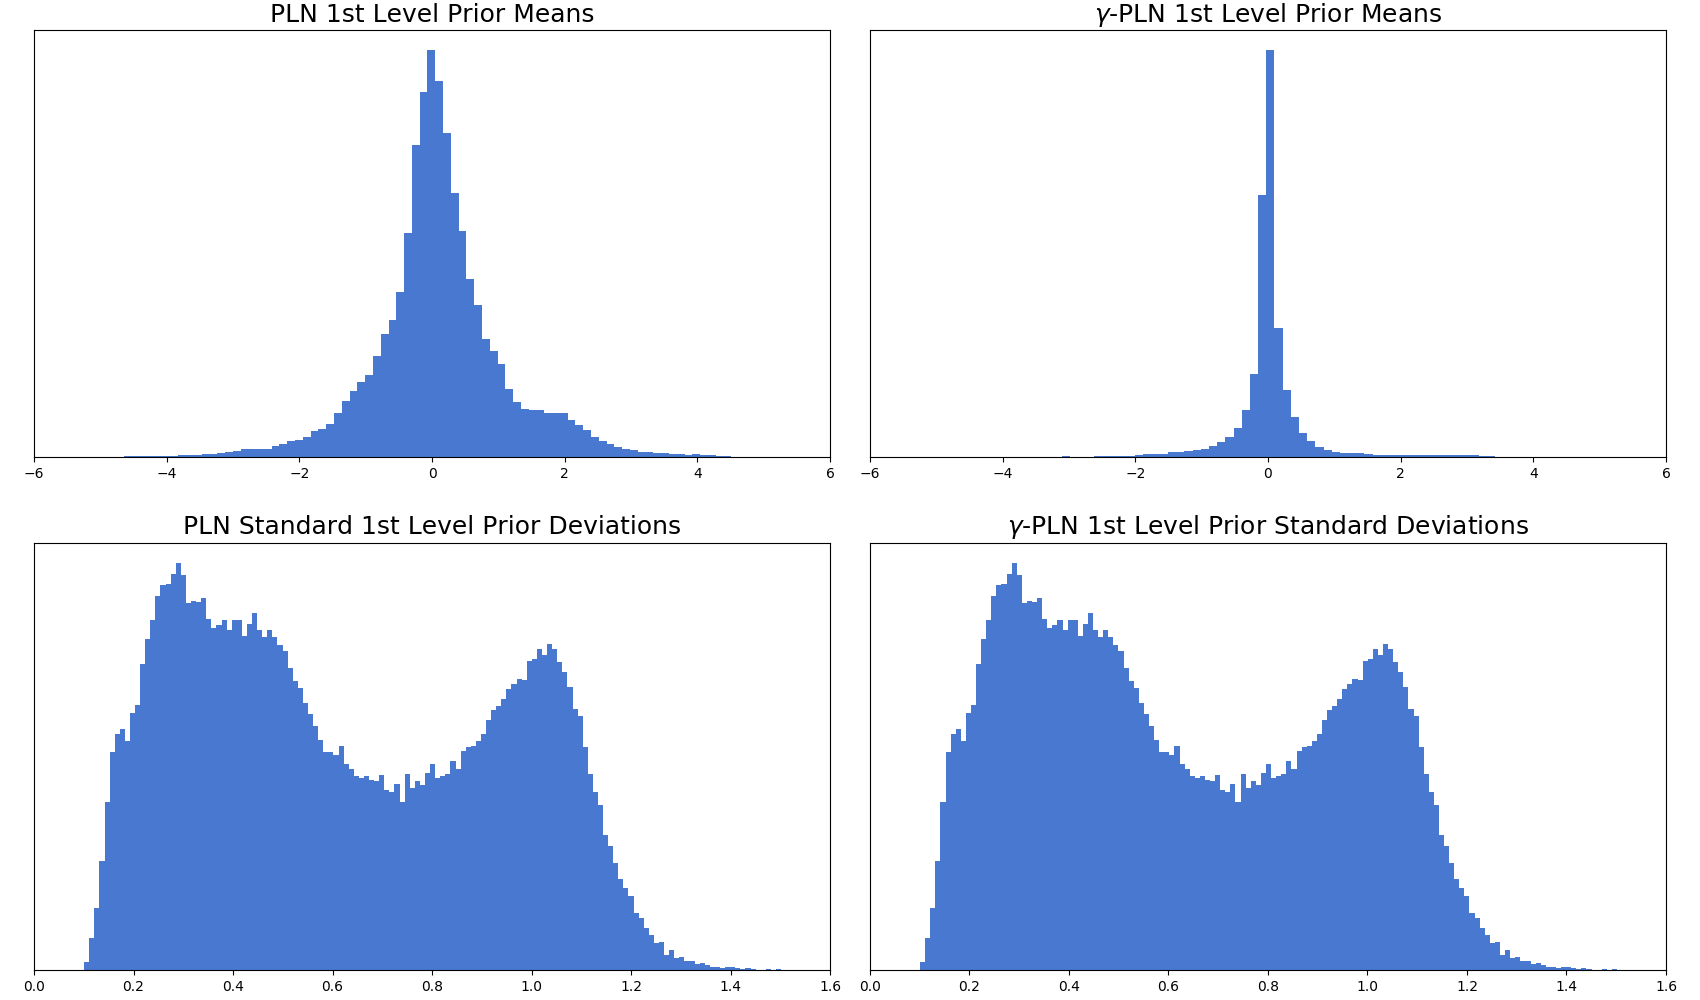
\includegraphics[width=\textwidth]{ladder_gamma_p1_comp.png}
  \caption{ladder on kodim21}
  \label{fig:ladder_gamma_p1_comp}
\end{figure}
\begin{figure}[H]
  \centering
  
\includegraphics[width=\textwidth]{ladder_gamma_q1_comp.png}
  \caption{ladder on kodim21}
  \label{fig:ladder_gamma_q1_comp}
\end{figure}
\begin{figure}[H]
  \centering
  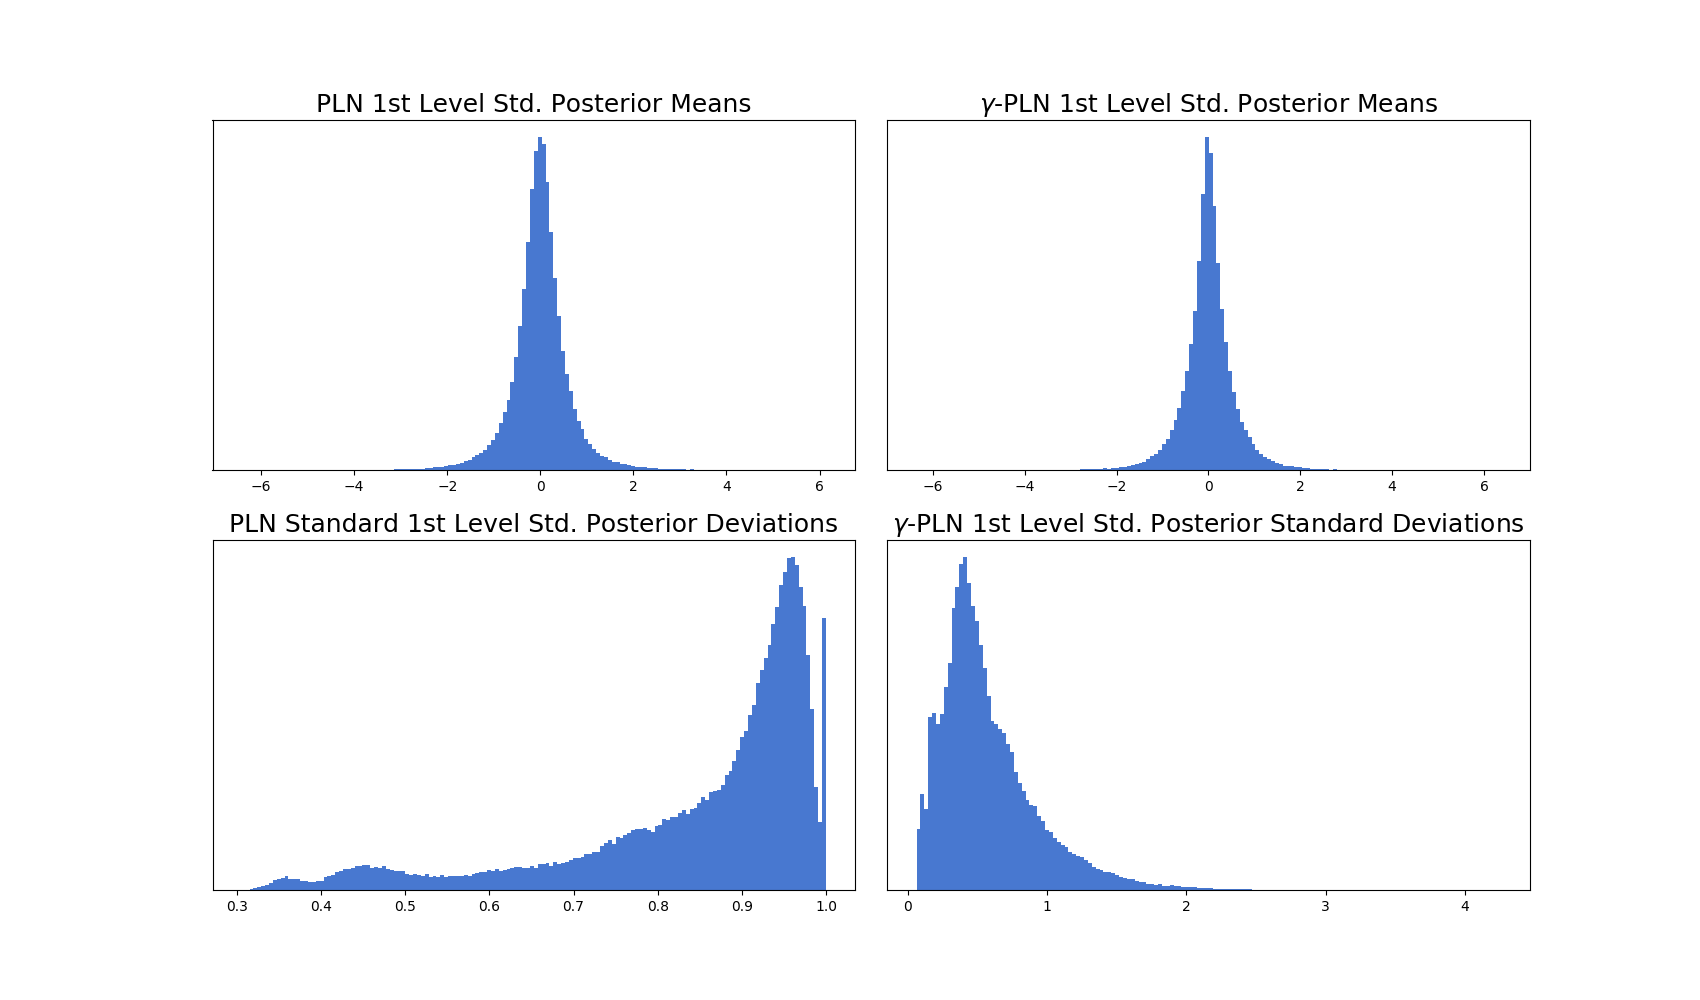
\includegraphics[width=\textwidth]{ladder_gamma_std_q1_comp.png}
  \caption{ladder on kodim21}
  \label{fig:ladder_gamma_std_q1_comp}
\end{figure}
\begin{figure}[H]
  \centering
  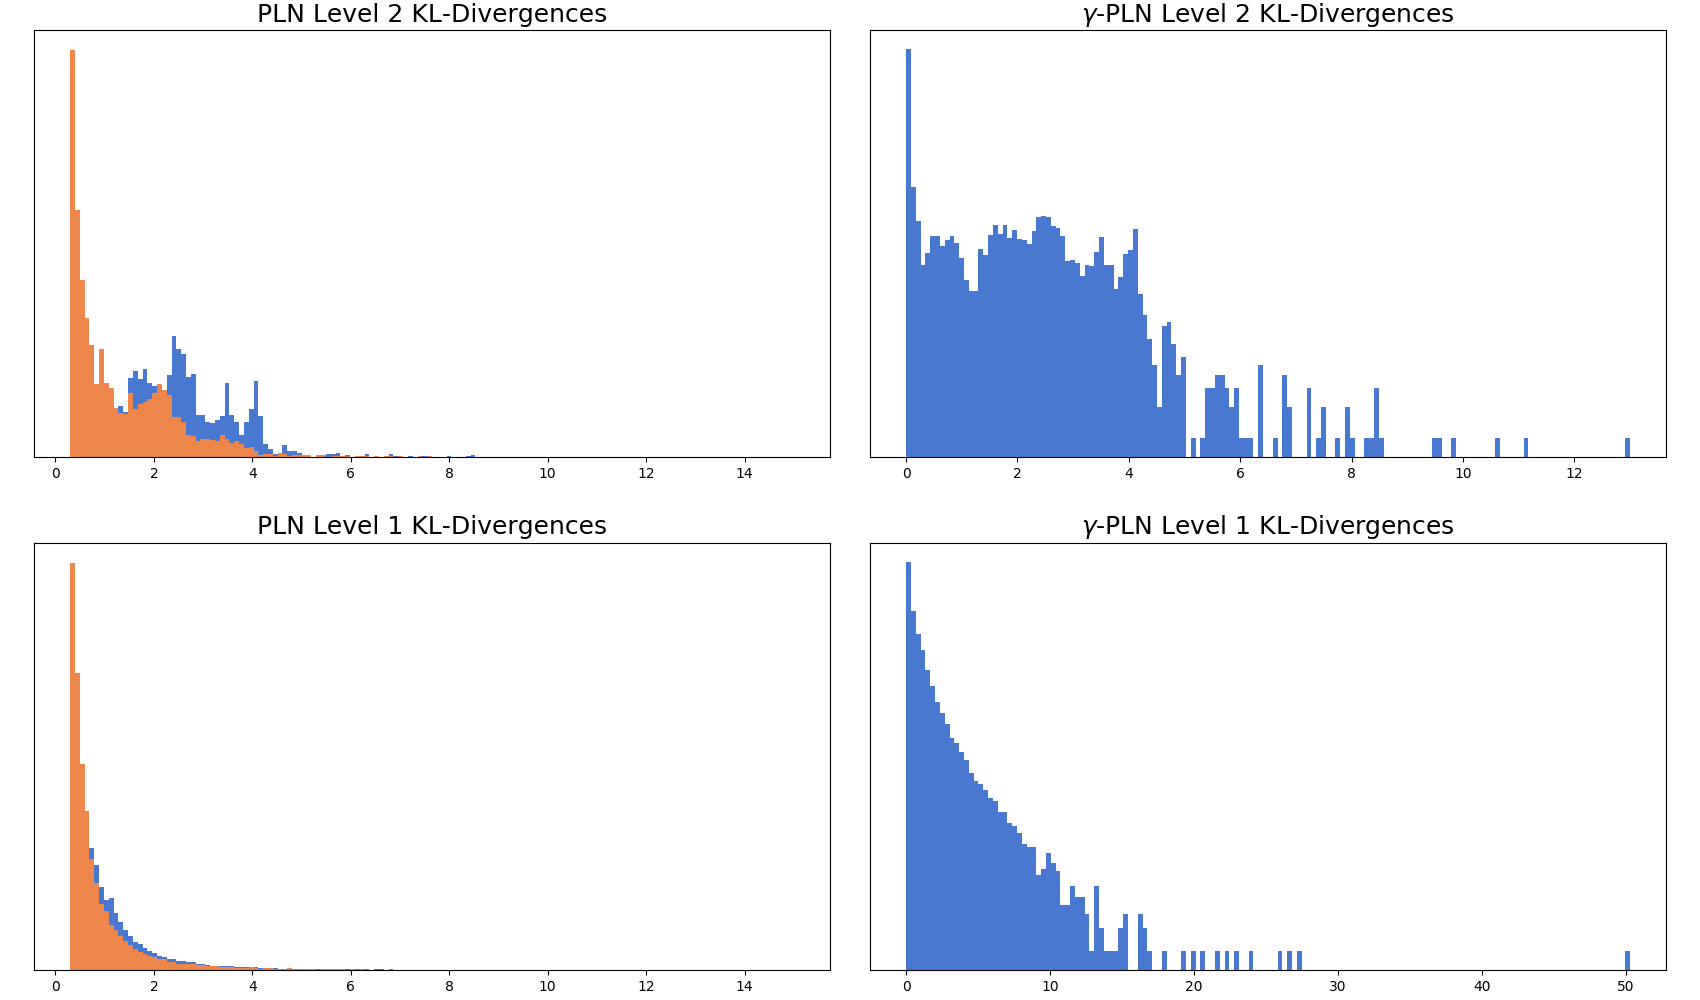
\includegraphics[width=\textwidth]{ladder_gamma_kl_comp.png}
  \caption{ladder on kodim21}
  \label{fig:ladder_gamma_kl_comp}
\end{figure}
\begin{figure}[H]
  \centering
  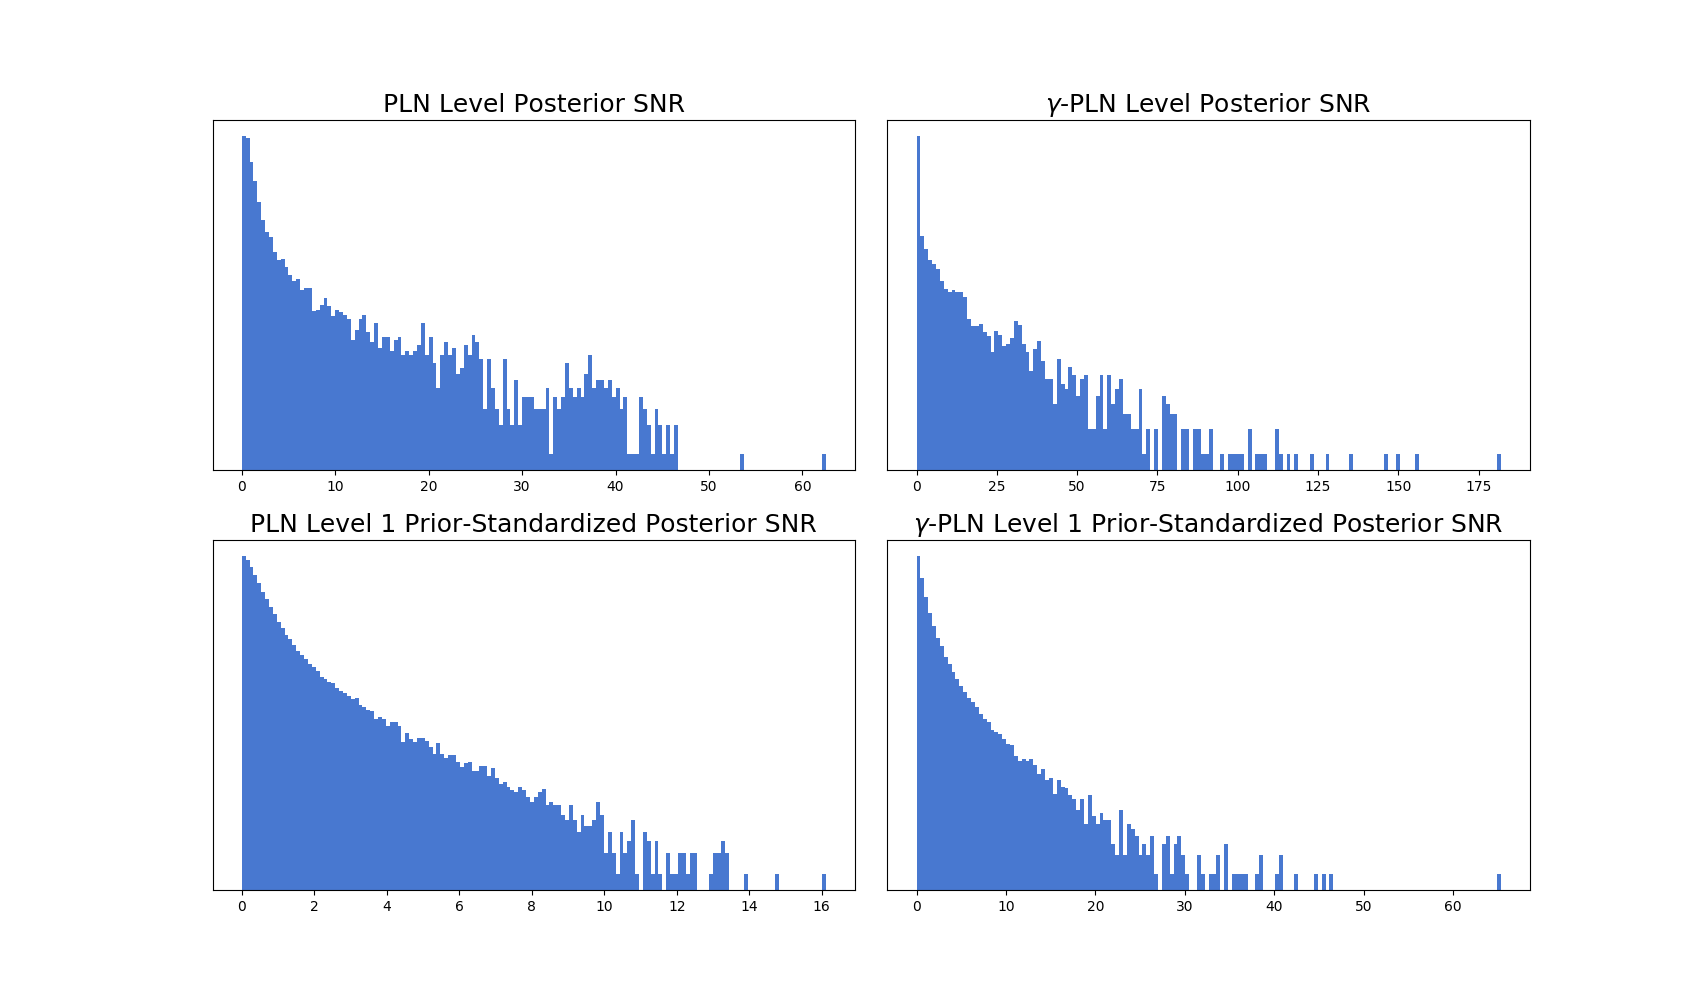
\includegraphics[width=\textwidth]{ladder_gamma_snr_comp.png}
  \caption{ladder on kodim21}
  \label{fig:ladder_gamma_snr_comp}
\end{figure}

\section{Compression Speed}
\par
Although not a focus of our project, we now briefly examine the the encoding and
decoding speed of our method. We have plotted the compression ratios of our
models against the time it took them to encode / decode them using IS-GS in
Figure \ref{fig:kodim01_coding_time}. As increasing the reconstruction quality
leads to higher KL divergences between the latent posteriors and priors, both the
importance sampler and the greedy sampler will need to split up a higher total
KL, and thus we expect the coding to become slower. This is precisely what we
observe, with a seemingly approximately linear growth, although we do not have
data to conclude this. We also see that encoding consistently takes around 3
times as long as decoding. It is clear that our method is not yet practical:
even the fastest case takes around a minute to encode and about 20 seconds to
decode, which very far away for real-time applications for now. The precise
values are reported in Table \ref{tab:kodim01_coding_time}.
\begin{figure}
  \centering
  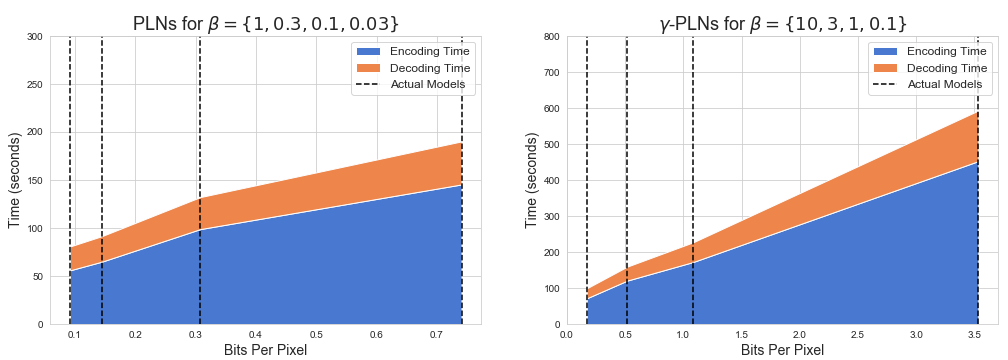
\includegraphics[width=\textwidth]{kodim01_coding_time.png}
  \caption{Coding times of models plotted agains their rates. \textbf{Left:}
    Regular PLNs. \textbf{Right:} $\gamma$-PLNs. The striped lines indicate
    the concrete positions of our models in the rate line. While it seems
    that there is a
    linear relationship between rate and coding time, we do not have enough
    datapoints to conclude this.}
  \label{fig:kodim01_coding_time}
\end{figure}

\begin{table}[]
  \centering
  \begin{tabular}{|r||c|c|c|c||c|c|c|c|}
    \hline
    & \multicolumn{4}{c||}{\textbf{PLNs}} & \multicolumn{4}{c|}{\textbf{$\gamma$-PLNs}} \\
    \hline 
    $\beta$ & 1 & 0.3 & 0.1 & 0.03 & 10 & 3 & 1 & 0.1 \\ 
    \hline\hline
    Encoding Time (s) & 55.91 & 64.95 & 98.85 & 145.38 & 71.40 & 120.54 & 172.34 & 452.49 \\
    \hline
    Decoding Time (s) & 24.85 & 26.61 & 33.34 & 44.85 & 27.81 & 38.87 & 54.86 & 140.52 \\
    \hline
  \end{tabular}
  \caption{haha}
  \label{tab:kodim01_coding_time}
\end{table}




% EXPERIMENT TODO:
% comparison of different sized images' coding
% Balle hyperprior efficiency plot
% Sonderby latent KL plot
% latent variance plot
